\chapter{Pruebas}

En este capítulo se va a analizar como se comporta la aplicación frente a un escenario real, con el fin de apreciar la fiabilidad con la que representa la potencia.
\\
\\
Para ello se han realizado unas mediciones con la aplicación en una máquina 'multipower' (smith machine), utilizando una escala para medir la distancia con respecto al tiempo, haciendo uso de una cámara (no de alta velocidad). Se ha a procedido a calcular la velocidad real media y la velocidad calculada, con el fin de ver cual es la diferencia. Puesto que el cálculo de la velocidad es el que más error implica en nuestro sistema.

\begin{figure}[H]
	\centering
	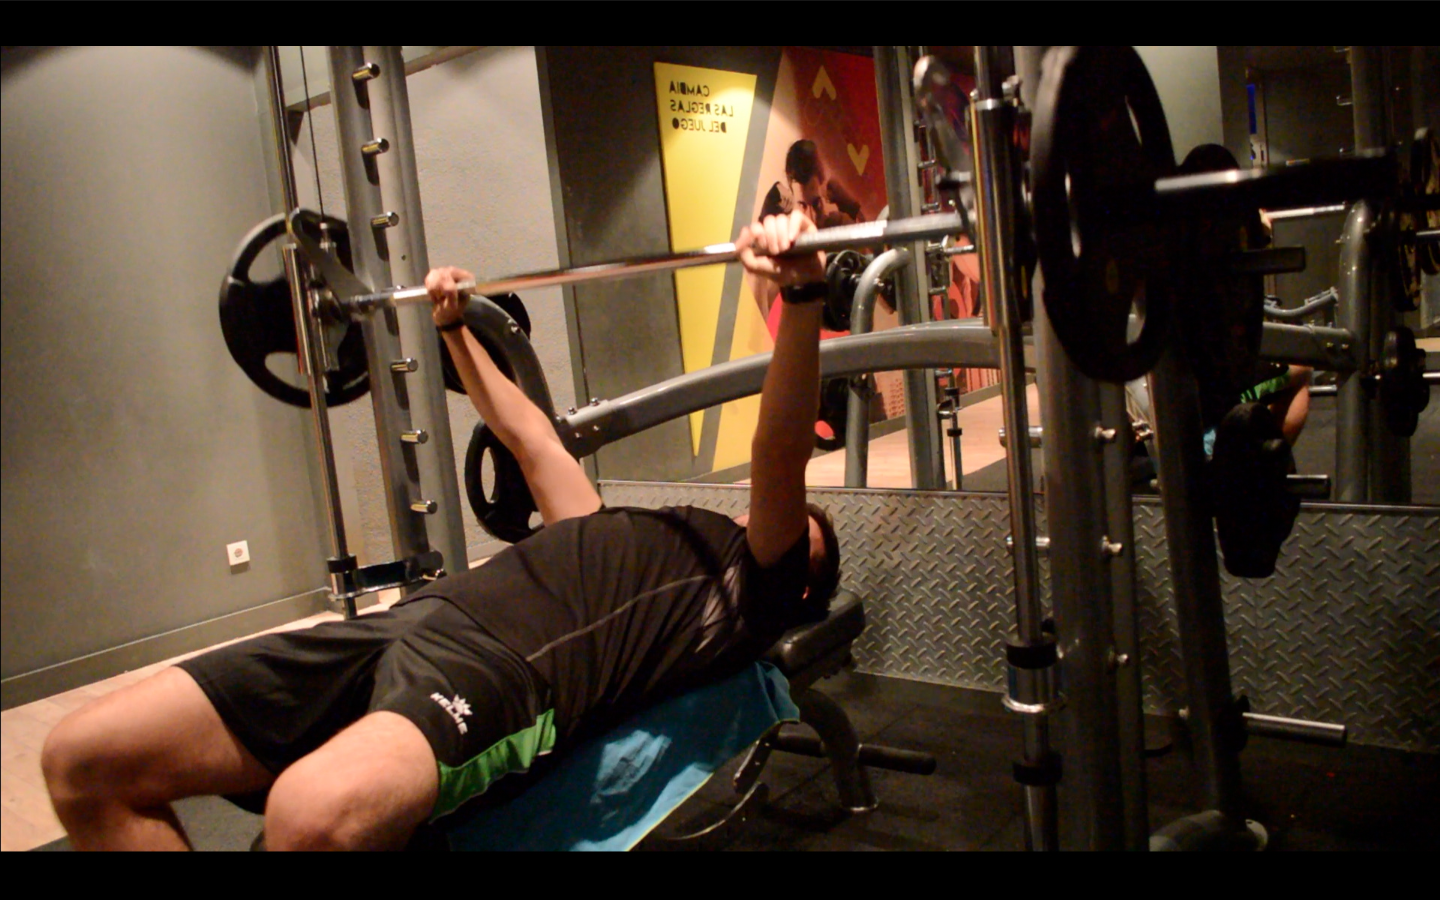
\includegraphics[scale=0.2]{imagenes/prueba1.png}
	\caption{Realización del primer test de la aplicación.}
	\label{Realización test}
\end{figure}

\section*{Test 1}

Se realizó una serie con 3 repeticiones.


\begin{table}[H]
\centering
\caption{Test 1}
\label{Test 1}
\begin{tabular}{|l|l|l|l|}
\hline
Tiempo (s) & Velocidad media real (m/s) & Velocidad media calculada (m/s) & Diferencia \\ \hline
1          & 0,175                      & 0                               & 0,175      \\ \hline
2          & 0,175                      & 0,11                            & 0,065      \\ \hline
3          & 0,175                      & 0,19                            & 0,015      \\ \hline
4          & 0,08                       & 0,21                            & 0,1225     \\ \hline
5          & 0,08                       & 0,35                            & 0,27       \\ \hline
6          & 0,262                      & 0,35                            & 0,08       \\ \hline
7          & 0,087                      & 0,76                            & 0,67       \\ \hline
8          & 0,22                       & 0,28                            & 0,06       \\ \hline
9          & 0,17                       & 0,28                            & 0,11       \\ \hline
10         & 0,25                       & 0,43                            & 0,18       \\ \hline
\end{tabular}
\end{table}

\section*{Test 2}

Esta vez se realizó una sola repetición. Para evaluar el comportamiento de la aplicación a baja velocidad.

\begin{table}[H]
\centering
\caption{Test 2}
\label{Test 2l}
\begin{tabular}{|l|l|l|l|}
\hline
Tiempo (s) & Velocidad media real (m/s) & Velocidad media calculada (m/s) & Diferencia \\ \hline
1          & 0                          & 0                               & 0          \\ \hline
2          & 0                          & 0                               & 0          \\ \hline
3          & 0                          & 0,190                           & 0,190      \\ \hline
4          & 0                          & 0,26                            & 0,26       \\ \hline
5          & 0,05                       & 0,26                            & 0,21       \\ \hline
6          & 0,10                       & 0,26                            & 0,16       \\ \hline
7          & 0,076                      & 0,15                            & 0,12       \\ \hline
8          & 0,05                       & 0,15                            & 0,10       \\ \hline
9          & 0,05                       & 0,15                            & 0,10       \\ \hline
10         & 0,03                       & 0,27                            & 0,24       \\ \hline
\end{tabular}
\end{table}

\section*{Test 3}

Se realizaron 15 repeticiones a lo largo de 40 segundos. Evaluando así el comportamiento de la aplicación en series largas.

\begin{table}[H]
\centering
\caption{Test 3}
\label{Test 3}
\begin{tabular}{|l|l|l|l|}
\hline
Tiempo (s) & Velocidad media real (m/s) & Velocidad media calculada (m/s) & Diferencia \\ \hline
0          & 0                          & 0                         & 0          \\ \hline
5          & 0.66                       & 0.57                      & 0,09       \\ \hline
10         & 0,96                       & 0,61                      & 0,35       \\ \hline
15         & 0,56                       & 1,43                      & 0,87       \\ \hline
20         & 0,54                       & 1,16                      & 0,62       \\ \hline
25         & 0,24                       & 1,94                      & 1,7        \\ \hline
30         & 0,64                       & 2,00                      & 1,36       \\ \hline
35         & 0,76                       & 2,31                      & 1,55       \\ \hline
40         & 0,40                       & 2,04                      & 1,64       \\ \hline
\end{tabular}
\end{table}

\noindent
Se puede ver que la aplicación se comporta de manera correcta en tiempo real, sin retardo apreciable por el usuario. Sin embargo la aplicación parece ser poco precisa cuando la velocidad del ejercicio es muy baja y cuando se produce desaceleración. Además la diferencia entre los valores calculados y reales aumenta con el tiempo, produciendo así un error bastante elevado. Esto es debido a que la estimación de la velocidad actual por medio de la integración diverge alejandose de la realidad rápidamente debido al ruido.
\\
\\
A falta de más pruebas, la aplicación es funcional, aunque su cálculo de la potencia es aproximado y contiene un gran margen de error. Por lo que no podemos garantizar que la aplicación realice la monitorización de manera correcta, especialmente cuando el tiempo de la serie es elevado.
